% uid: ""
% school: "college"
% level: "7eme"
% chapter: "التناظر المحوري"
% chapter_slug: "symetrie-axiale"
% title: "منصّف زاوية ومحور تناظرها"
% difficulty: "Facile"
% tags: ["symetrie-axiale", "bissectrice", "angle", "perimetre"]
% provenance: "own"
% batch: "2026-11-27-symetrie-axiale-7eme"
% Exercice 9/10 de la série 7ème « التناظر المحوري » (statement + \axsol + solution). Compiler avec XeLaTeX + axiomath.sty (+ axiomaths-logo.png).
\documentclass[12pt,a4paper]{article}
\usepackage[level=7b,color=0F766E]{axiomath}
\newcommand{\cm}{\,\mathrm{cm}}
\axsetup{title={التناظر المحوري}, corrige}

\begin{document}

\begin{corr}[title={منصّف زاوية ومحور تناظرها}, stars=2, source={Axiomaths}]
$\widehat{xOy}$ زاوية قيسها $70^\circ$ و $[Oz)$ منصّفها. $A$ نقطة من $[Ox)$ حيث $OA=3\cm$ ، و $B$ نقطة من $[Oz)$ ، و $A'$ مناظرة $A$ بالنسبة إلى المستقيم $(Oz)$.
\begin{enumerate}
  \item ابنِ الشكل ثم احسب $\widehat{xOz}$.
  \item بين أن $A'$ تنتمي إلى $[Oy)$ ثم احسب $OA'$.
  \item قارن $BA$ و $BA'$.
  \item ما هو مناظر المثلث $OAB$ بالنسبة إلى $(Oz)$ ؟ قارن محيطي المثلثين $OAB$ و $OA'B$.
\end{enumerate}
\axsol
\begin{enumerate}[itemsep=14pt]
  \item $[Oz)$ منصّف $\widehat{xOy}$ ، فهو يقسمها إلى زاويتين متقايستين :
  \[\widehat{xOz}=\dfrac{70^\circ}{2}=35^\circ\]
  \begin{center}
  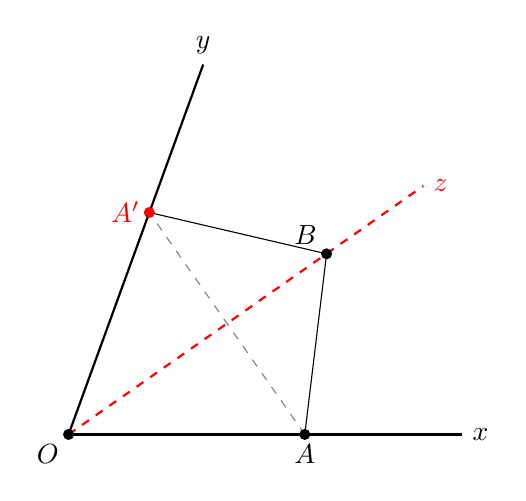
\begin{tikzpicture}[scale=1]
    \draw[thick] (0,0)--(5,0) node[right] {$x$};
    \draw[thick] (0,0)--(1.710,4.698) node[above] {$y$};
    \draw[thick,red,dashed] (0,0)--(4.505,3.155) node[right] {$z$};
    \draw (3,0)--(3.277,2.294)--(1.026,2.819);
    \draw[dashed,gray] (3,0)--(1.026,2.819);
    \fill (0,0) circle (2pt) node[below left] {$O$};
    \fill (3,0) circle (2pt) node[below] {$A$};
    \fill[red] (1.026,2.819) circle (2pt) node[left] {$A'$};
    \fill (3.277,2.294) circle (2pt) node[above left] {$B$};
  \end{tikzpicture}
  \end{center}
  \item\leavevmode
  \begin{prop}[منصّف زاوية]
  \ib{المستقيم الحامل لمنصّف زاوية هو محور تناظر لها} : المناظر بالنسبة إليه للنصف مستقيم $[Ox)$ هو $[Oy)$.
  \end{prop}
  $A$ تنتمي إلى $[Ox)$ ، إذن مناظرتها $A'$ تنتمي إلى مناظر $[Ox)$ ، أي \ib{$A'\in[Oy)$}.

  $O$ تنتمي إلى المحور، فمناظرتها $O$. والتناظر يحافظ على الأطوال :
  \[OA'=OA=3\cm\]
  \item $B$ تنتمي إلى المحور $(Oz)$ ، فمناظرتها $B$ نفسها. التناظر يحوّل $[BA]$ إلى $[BA']$ ، إذن :
  \[\ib{$BA'=BA$}\]
  \item التناظر يحوّل $O$ إلى $O$ و $A$ إلى $A'$ و $B$ إلى $B$ : مناظر المثلث $OAB$ هو \ib{المثلث $OA'B$}.

  أضلاع المثلثين متقايسة مثنى مثنى ($OA'=OA$ ، $BA'=BA$ ، $OB=OB$) ، إذن \ib{لهما نفس المحيط}.
\end{enumerate}
\end{corr}

\end{document}
